\documentclass[tikz,border=3pt]{standalone}
\usepackage{xcolor}
\usetikzlibrary{arrows.meta,decorations.pathmorphing,positioning}
\definecolor{pulseblue}{HTML}{2563EB}
\definecolor{devicegray}{HTML}{64748B}
\definecolor{devicefill}{HTML}{F1F5F9}
\begin{document}
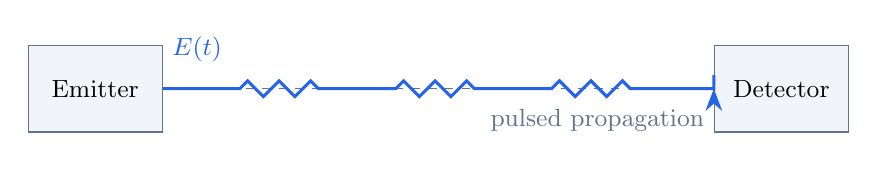
\begin{tikzpicture}[>=Stealth,every node/.style={font=\small}]
  \node[draw=devicegray,fill=devicefill,minimum width=1.7cm,minimum height=1.1cm] (source) {Emitter};
  \node[draw=devicegray,fill=devicefill,minimum width=1.7cm,minimum height=1.1cm,right=7cm of source] (sensor) {Detector};
  \draw[devicegray,dashed] (source.east) -- (sensor.west);
  \draw[pulseblue,line width=1.1pt,-Stealth,decorate,
    decoration={straight zigzag,meta-segment length=10mm,segment length=4mm,amplitude=1mm}]
    (source.east) -- (sensor.west);
  \node[pulseblue,above=5mm of source.east,anchor=west] {$E(t)$};
  \node[devicegray,below=4mm of sensor.west,anchor=east] {pulsed propagation};
\end{tikzpicture}
\end{document}
